\documentclass[a4paper]{article}
\usepackage[spanish]{babel}
\usepackage{hyperref}
\usepackage{graphicx}
\usepackage{fancyhdr}
\usepackage[margin=3.5cm, top=2.5cm, bottom=3cm, includefoot]{geometry}
\usepackage{xcolor}


\graphicspath{ {imagenes2/} }

\setlength{\headsep}{2.5cm}
\pagestyle{fancy}
\fancyhf{}
\lhead{
\includegraphics[width=4cm]{Nuevo-Logo-1.jpg}}
\rfoot{{\textbf{Spark} \\ Master en Big Data y Data Science}}
\lfoot{ \break Página \thepage}
\renewcommand{\headrulewidth}{0pt}





\begin{document}
\begin{titlepage}
    \centering
    {\bfseries\LARGE Universidad Internacional de Valencia \par}
    \vspace{1cm}
    {\scshape\Large Master en Big Data y Data Science \par}
    \vspace{3cm}
    {\scshape\Huge Problema 2: Categoría de video menos vista \par}
    \vspace{1cm}
    \begin{figure}[h]
        \centering
        
\includegraphics[width=8cm, keepaspectratio]{Nuevo-Logo-1.jpg}

    \end{figure}
    \vspace{1cm}
    {\itshape\Large Procesamiento de datos masivos: Spark \par}
    \vspace{3cm}
    {\Large Autor: \par}
    {\Large Adrián Hernández Padrón \par}
    {\Large Julio 2022 \par}


\end{titlepage}
\clearpage
\begin{section}{Código}
Una vez hemos leido los datos de entrada, vamos a mapearlos con un flatMap. Debido a la naturaleza del archivo no es necesario leer las filas una a una, podemos añadir las columanas deseadas con un .split y el índice de la columna.
Es necesario hacer un try-except para evitar almacenar datos vacíos, con esto solucionamos que el reduceByKey de problemas ya que no sabe como actuar con filas vacías. 

\begin{figure}[h]
    \centering
    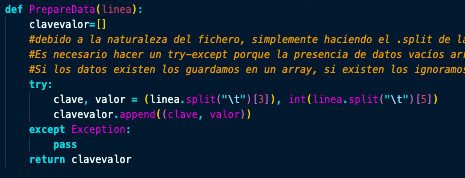
\includegraphics[width=\textwidth, keepaspectratio]{codigo1}
    \caption{Devolvemos la clave-valor con la categoría-tiempo de reproducción.}
\end{figure}

El reduceByKey que hace la suma de todos los minutos de reproducción para cada categoría, lo hacemos con lambda y después calculamos el valor mínimo entre todas las categorías.
\begin{figure}[h]
    \centering
    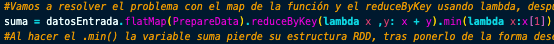
\includegraphics[width=\textwidth, keepaspectratio]{codigo2}
  
\end{figure}

El valor devuelto, que es el mínimo, pierde su estructura RDD, por tanto una vez lo coloquemos con la estructura deseada de salida, usamos .parallelize para transformarlo a RDD y poder usar saveAsTextFile.
\begin{figure}[h]
    \centering
    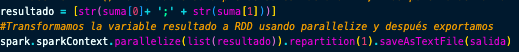
\includegraphics[width=\textwidth, keepaspectratio]{codigo3.png}
\end{figure}

\end{section}
\clearpage
\begin{section}{Ejecución y resultados}
    Para lanzar el programa escribimos lo siguiente por la línea de comandos, en donde 0222 es la carpeta con todos los archivos de texto y el *.txt indica que queremos leer todos los archivos txt de la carpeta.
    $spark-submit CategoriaDeVideosMenosVista.py 'file:/Users/adrihp/Master/MBID03/scriptsSpark/0222/*.txt' file:/Users/adrihp/Master/MBID03/scriptsSpark/salida2$
    No es necesario eliminar el archivo txt que no contiene datos puesto que con el try-except se ignora sin generar ningún problema.
    
    La entrada tiene la siguiente estrucutra y la salida se guarda en la carpeta salida2 y tiene la siguiente estructura.
    \begin{figure}[h]
        \centering
        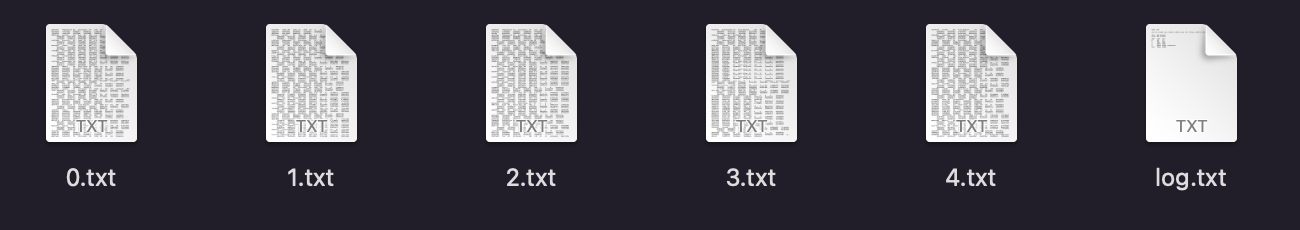
\includegraphics[width=\textwidth, keepaspectratio]{entrada21.png}
        \caption{Carpeta con la entrada.}

    \end{figure}
    \begin{figure}[h]
        \centering
        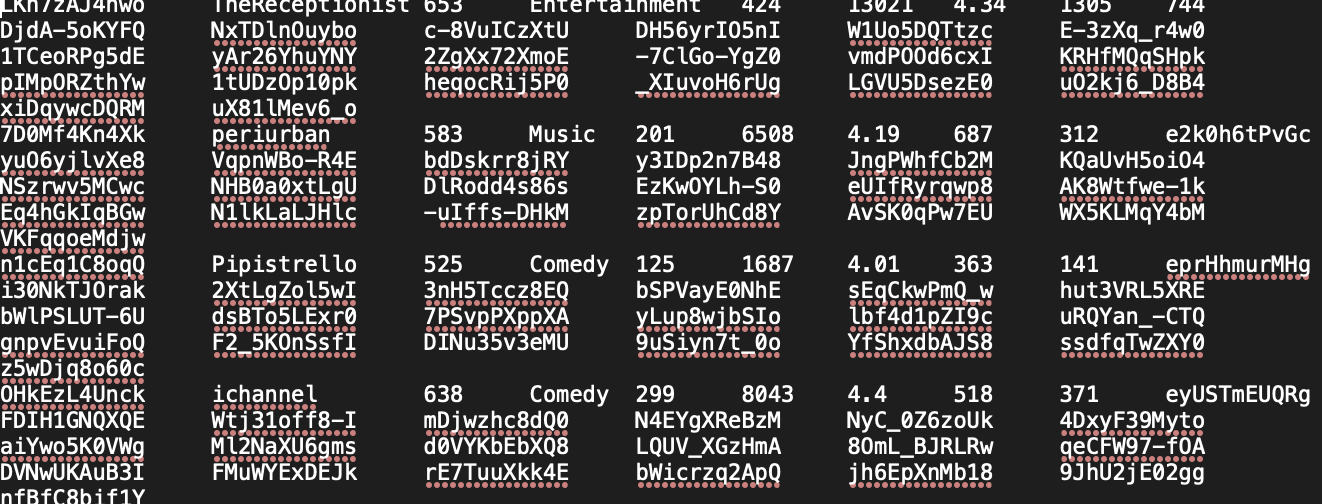
\includegraphics[width=\textwidth, keepaspectratio]{entrada2.png}
        \caption{Entrada: ejemplo de un fichero}

    \end{figure}
    \begin{figure}[h]
        \centering
        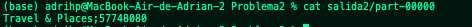
\includegraphics[width=\textwidth, keepaspectratio]{salida2.png}
        \caption{Salida: Categoría de video;Tiempo de reproducción total}

    \end{figure}
\end{section}
\end{document}  